\section{Portfolio revision implementation}
The portfolio revision model is an extension of the CVaR model to revise and evaluate portfolios after some time has past.
In this work, is assumed that four weeks are gone and the previous portfolio on section~\ref{sec:CVaR} could no longer be credible and acceptable.
So, a revision of the portfolio on the (2008-03-28) to maximize the return under two different strategies (risk averse and risk neutral) are considered.
The portfolio revision entails some costs for the transactions deviations on the portfolio.
In this way, is assumed a transaction cost of 0.1\% of the traded amount in kr., assuming at least 50 kr per trade.

The portfolio revision model is defines as
\begin{align}
\up{TotalCost} &= \lambda \up{CVaR} - {\left( 1 - \lambda \right)} \up{MeanReturn} + \up{TradeCost} \\
x^\up{old}_{i} + x^\up{difference}_{i} &= x_{i} \; \; \forall i \\
\sum_{i} x^\up{old}_{i} &= \sum_{i} x_{i} \\
x^\up{difference}_{i} &\le B_{i} \up{M} \; \; \forall i \\
-x^\up{difference}_{i} &\le B_{i} \up{M} \; \; \forall i \\
\up{TradeCost} &= \sum_{i} \up{TC}_{i} \\
\up{TC}_{i} &\ge B_{i} \up{penalty} \; \; \forall i \\
\up{TC}_{i} &\ge 0.001 x^\up{difference}_{i} \; \; \forall i \\
\up{TC}_{i} &\ge - 0.001 x^\up{difference}_{i} \; \; \forall i \\
\end{align}
where $\lambda$ is the level of risk of the strategy (1 - Risk Averse ; 0 - Risk Neutral), TradeCost is the total cost of the trades of all changes in portfolio, and $x^\up{old}_{i}$ is the previous result of portfolio updated with the current historical monthly return.
In this way, the first $x^\up{old}_{i}$ is based on the results of section~\ref{sec:CVaR} considering the run related to risk averse.
The difference between the $x^\up{old}_{i}$ and the new $x_{i}$ is given by $x^\up{difference}_{i}$.
$B_{i}$ is a binary variable to characterize if there are or not a transacation by each ETF $i$, and M is a high constant value to allow the selection of trade or not trade.
$\up{TC}_{i}$ is the tradde cost by each ETF $i$, and penalty corresponds to the trade cost of 50 kr.
In addition to the previous constraints, the CVaR model presented in section~\ref{sec:CVaR} is considered as constraints in the portfolio revision model.

The aim of the present section is to minimize the TotalCost of the full portfolio revision model for each type of strategy (risk averse and risk neutral).
The results concerning the expected value, CVaR and assets portfolio are presented in Table\ref{tbl:portfoliotabel} considering a comparison between the different strategies and the initial solution. 

Results...




\begin{figure}[tp]
\centering
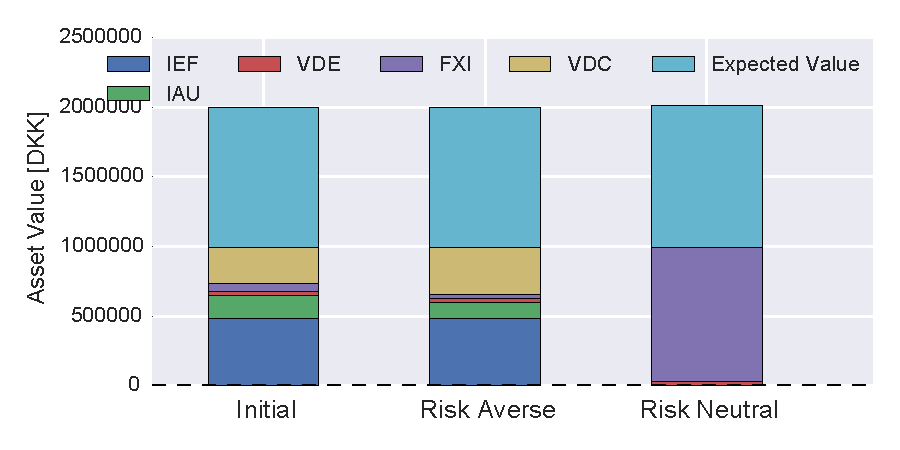
\includegraphics{../pic/portfoliorevision_portfolio.pdf}
\caption{Initial portfolio versus those found by the two types of traders.}
\label{fig:prevpf}
\end{figure}

\begin{table}
\caption{Stats for portfolios found by portfolio revision model.}\label{tbl:portfoliotabel}
\centering
\begin{tabular}{lrrr}
\toprule
{} &  Expected Profit &      CVaR &  Trading Cost \\
\midrule
Type         &                  &           &               \\
Initial      &          8423.76 &   3436.86 &          0.00 \\
Risk Averse  &          6545.42 &   2469.89 &        214.37 \\
Risk Neutral &         24735.63 &  36958.75 &       1820.37 \\
\bottomrule
\end{tabular}

\end{table}